\section{我们的方法}
\label{sec:pure-traction}

本节对应 \code{vbot} 的 \code{dev1-pure-traction} 分支，提交为 \code{1810875}。纯牵引方案训练状态估计器和速度策略，直接生成前向、侧向和偏航速度指令。\ev{C14}

\subsection{网络设计}
网络层宽与反馈路径见图~\ref{fig:pure-traction-network}。
\begin{itemize}
  \item \textbf{状态估计器}\enspace 用最近 6 帧本体观测（270 维）估计机身线速度、外力和力矩（归一化，各 3 维）。
  \item \textbf{速度策略}\enspace 最新观测、估计量与 $(D,\tau)$ 组成 $45+9+2=56$ 维输入。参数归一化至 $[-1,1]$，估计量截断梯度。
  \item \textbf{策略原始输出}\enspace 训练时从对角高斯分布采样 $\bm u_t$，评估与部署时取均值。
  \item \textbf{指令后处理}\enspace $\mathcal P$ 先按前向 $[-0.5,1.3]$、侧向 $[-0.5,0.5]$（$\mathrm{m/s}$）和偏航 $[-1.5,1.5]$（$\mathrm{rad/s}$）限幅。平移范数 $\le 0.05\,\mathrm{m/s}$ 或偏航绝对值 $\le 0.05\,\mathrm{rad/s}$ 时清零对应分量。
  \item \textbf{下一帧反馈}\enspace Policy8 使用当前观测中的 $\bm c_t$。本步输出 $\bm c_{t+1}=\mathcal P(\bm u_t)$ 按图中的 $S$ 缩放后写入下一帧。
\end{itemize}

\begin{figure}[!htbp]
\centering
\begin{tikzpicture}[
  block/.style={draw=ink,fill=ink!4,rounded corners=2pt,
    align=center,inner sep=4pt,font=\small},
  input/.style={block,minimum height=19mm},
  estimate output/.style={block,text width=12mm,minimum height=8mm,
    inner sep=1.4pt,font=\footnotesize},
  >={Stealth[length=2mm]},line width=0.7pt
]
\node[block,text width=73mm,minimum height=14mm] (history) at (-16mm,0)
  {\textbf{本体观测历史}\quad $h_t$（6 帧，270 维）\\[2pt]
   最新帧含缩放后的当前执行指令 $S\bm c_t$};

\node[input,text width=28mm] (base) at (-58mm,-25mm)
  {\textbf{冻结 Policy8}\\[2pt]关节动作 $\bm a_t$\\（12 维）};
\node[input,text width=36mm] (estimate) at (-17mm,-25mm)
  {\textbf{状态估计器}\\[2pt]
   \mbox{\scriptsize $270\!\to\!512\!\to\!256\!\to\!128\!\to\!9$}\\[2pt]
   {\footnotesize 归一化输出（9 维）}};
\node[input,text width=27mm] (latest) at (23mm,-25mm)
  {\textbf{最新帧观测}\\[2pt]$\bm o_t$（45 维）};
\node[input,text width=27mm] (parameters) at (61mm,-25mm)
  {\textbf{参考参数}\\[2pt]$(D,\tau)$ 归一化\\（2 维）};

\node[estimate output] (velocity) at (-33mm,-42.5mm) {线速度\\3 维};
\node[estimate output] (force) at (-17mm,-42.5mm) {外力\\3 维};
\node[estimate output] (moment) at (-1mm,-42.5mm) {力矩\\3 维};

\node[block,text width=28mm,minimum height=17mm] (simulation) at (-58mm,-60mm)
  {\textbf{仿真执行}\\[2pt]获取下一帧本体状态};
\node[block,fill=ink!8,text width=96mm,minimum height=15mm] (actor) at (23mm,-60mm)
  {\textbf{速度策略 MLP}\quad $56\to256\to128\to64\to3$\\[2pt]
   输出前向、侧向、偏航速度均值};
\node[block,text width=96mm,minimum height=15mm] (process) at (23mm,-80mm)
  {\textbf{限幅与死区}\\[2pt]
   训练时采样，推理时取均值，再处理原始指令 $\bm u_t$\\[2pt]
   $\bm c_{t+1}=\mathcal P(\bm u_t)$};
\node[block,text width=128mm,minimum height=14mm] (next) at (-4mm,-106mm)
  {\textbf{更新下一帧观测}\quad
   $\bm o_{t+1}[0{:}3]=S\bm c_{t+1}$，$S=\operatorname{diag}(2,2,0.25)$\\[2pt]
   将新观测加入历史 $h_{t+1}$};

\draw[->] ([xshift=-30mm]history.south) -- ++(0,-4mm) -| (base.north);
\draw[->] ([xshift=-1mm]history.south) -- (estimate.north);
\draw[->] ([xshift=29mm]history.south) -- ++(0,-4mm) -| (latest.north);
\draw[->] (base.south) -- (simulation.north);
\coordinate (estimate-split) at (-17mm,-36.5mm);
\draw (estimate.south) -- (estimate-split);
\draw[->] (estimate-split) -| (velocity.north);
\draw[->] (estimate-split) -- (force.north);
\draw[->] (estimate-split) -| (moment.north);
\coordinate (estimate-merge) at (-17mm,-48.8mm);
\draw (velocity.south) |- (estimate-merge);
\draw (force.south) -- (estimate-merge);
\draw (moment.south) |- (estimate-merge);
\draw[->] (estimate-merge) -- node[right,font=\scriptsize] {截断梯度} ([xshift=-40mm]actor.north);
\draw[->] (latest.south) -- (actor.north);
\draw[->] (parameters.south) -- ([xshift=38mm]actor.north);
\draw[->] (actor.south) -- (process.north);
\draw[->] (simulation.south) -- ([xshift=-54mm]next.north);
\draw[->] (process.south) -- ([xshift=27mm]next.north);
\coordinate (loop) at (79mm,0);
\draw[->,dashed,draw=ink!65] (next.east) -- (loop |- next.east) -- (loop)
  -- node[above,font=\footnotesize] {进入下一控制步} (history.east);
\end{tikzpicture}

\caption{网络架构}
\label{fig:pure-traction-network}
\end{figure}

\subsection{训练环境与采样}
\begin{itemize}
  \item \textbf{训练环境}\enspace 在 Vita01evt 粗糙地形仿真中训练，冻结 Policy8 运动底座，控制周期为 $0.02\,\mathrm{s}$。
  \item \textbf{回合类别}\enspace 按 $25\%$ 无力、$25\%$ 弱力、$50\%$ 常规牵引分配回合。无力回合全程施力为零。
  \item \textbf{施力时序}\enspace 弱力和常规牵引回合默认每 $10\,\mathrm{s}$ 重采一次世界系外力，保持 $7\,\mathrm{s}$，再清零 $3\,\mathrm{s}$。
  \item \textbf{弱力采样}\enspace 幅值均匀采自 $[0,10)\,\mathrm N$，方向在单位球面均匀采样。
  \item \textbf{常规牵引采样}\enspace 三个世界系力分量独立均匀采自 $[-40,40)\,\mathrm N$。
  \item \textbf{施力方式}\enspace 作用点 $\bm r^b$ 在机身原点前方 $0.17287\,\mathrm m$。按式~\eqref{eq:force-transform} 将外力转为机身系 $\bm F_t^b$，在质心施加该力和力矩 $(\bm r^b-\bm r_{\rm CoM}^b)\times\bm F_t^b$。其中 $\bm r_{\rm CoM}^b$ 为机身原点至质心的向量。\ev{C12}
  \item \textbf{监督标签}\enspace 使用机身系线速度、外力 $\bm F_t^b$ 和关于机身原点的力矩 $\bm r^b\times\bm F_t^b$。力标签和参考速度均由生成当前观测的控制段所施加的外力更新。
\end{itemize}

\subsection{由外力计算参考速度}

\subsubsection{质量--弹簧--阻尼模型}
设 $x$ 为参考位移，$x_0$ 为平衡位置。单轴虚拟质量--弹簧--阻尼模型在外力 $F$ 下满足
\begin{equation}
 M\ddot x+D\dot x+K(x-x_0)=F.
\end{equation}
\begin{itemize}
  \item \textbf{弹簧刚度 $K$}\enspace 产生指向平衡位置的恢复力。$K,D>0$ 时，恒力使位移 $x-x_0$ 趋于 $F/K$。
  \item \textbf{虚拟质量 $M$}\enspace 同一净力下，质量越大，加速度越小。从平衡位置静止起步时，初始加速度为 $F/M$。
  \item \textbf{阻尼 $D$}\enspace 产生与速度方向相反的力，耗散运动能量并使响应趋于稳定。
\end{itemize}

\subsubsection{平移参考速度}
\label{subsec:planar-reference}
纯牵引取 $K=0$，取消位置恢复力。令 $v=\dot x$，则 $M\dot v+Dv=F$。恒定有效拉力下，限幅前的参考速度趋于 $F/D$，时间常数为 $\tau=M/D$。两个平移轴共用 $D$ 和 $M=D\tau$。训练时按回合独立均匀采样 $D\in[15,30]\,\mathrm{N\,s/m}$ 和 $\tau\in[0.3,0.8]\,\mathrm s$。标准评估默认取 $D=20\,\mathrm{N\,s/m}$、$\tau=0.5\,\mathrm s$，对应 $M=10\,\mathrm{kg}$。\ev{C11,C15}

令 $\rho_t=\|\bm F_t^w\|_2$、$F_0=5\,\mathrm N$，以施加的三维外力幅值判定力阈值。有效平移力为
\begin{equation}
 \bm F^{b}_{xy,\mathrm{eff},t}
 = \left(1-\frac{F_0}{\max(\rho_t,F_0)}\right)\bm F^{b}_{xy,t}.
\end{equation}
\begin{samepage}
更新前，先将上一控制步的内部平面速度 $\bm s_{t-1}$ 转到当前航向。设 $\psi_t$ 为机身航向，$R(\cdot)$ 为二维旋转矩阵，$a=e^{-\Delta t/\tau}$，控制周期 $\Delta t=0.02\,\mathrm s$。力幅值低于阈值时清零内部状态，其余情况按式~\eqref{eq:exact} 做零阶保持离散更新
\begin{equation}
 \bm s_t=
 \begin{cases}
 aR(\psi_{t-1}-\psi_t)\bm s_{t-1}+(1-a)\bm F^{b}_{xy,\mathrm{eff},t}/D,
   & \rho_t\ge F_0,\\
 \bm 0, & \rho_t<F_0.
 \end{cases}
\end{equation}
\end{samepage}

\begin{samepage}
\subsubsection{偏航参考速度}
三维合力与机身系水平力均达到 $5\,\mathrm N$ 时启用偏航参考。水平力方向角为 $\theta_t=\operatorname{atan2}(F^b_{y,t},F^b_{x,t})$。默认偏航增益 $0.5\,\mathrm{s}^{-1}$ 乘以有符号的转向角误差，得到限幅前的偏航速度 $\omega^{*}_{z,t}$。通常选最短转向。当 $|\theta_t|\ge170^\circ$ 且已有转向选择时沿用该方向，必要时按 $2\pi-|\theta_t|$ 计算转角。最后用 $\mathcal P$ 处理平移与偏航，得到参考指令 $\bm c_{{\rm ref},t}$。图~\ref{fig:traction-reference-map} 给出稳态示例。\ev{C15}
\par
\end{samepage}

\begin{figure}[!htbp]
\centering
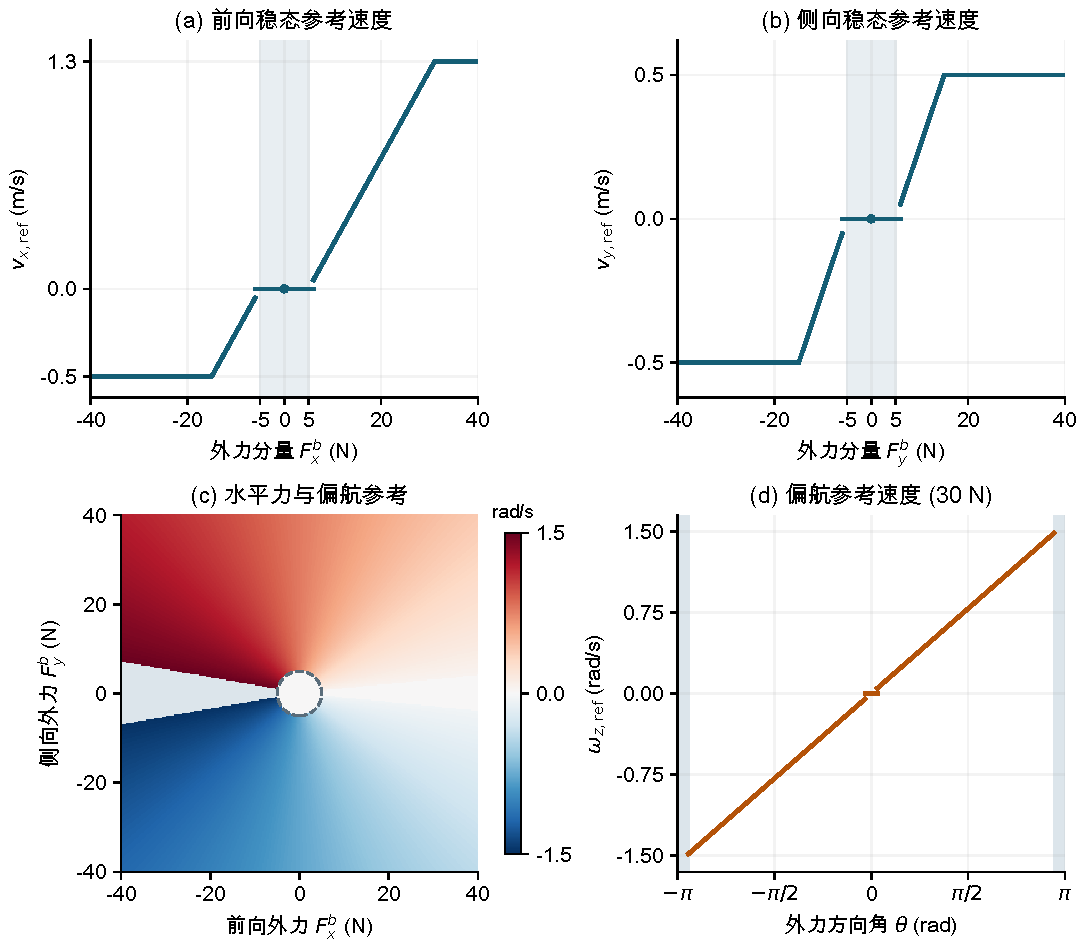
\includegraphics[width=0.76\linewidth]{figures/traction_reference_map.pdf}
\caption{纯牵引方案的外力与参考速度关系。取 $F_z^b=0$，$D=20\,\mathrm{N\,s/m}$。(a)、(b) 为单轴恒定施力时经后处理的稳态平移参考，(c)、(d) 为偏航参考的水平力分布和 $30\,\mathrm N$ 切片。后方灰区表示转向方向取决于历史选择。}
\label{fig:traction-reference-map}
\end{figure}

\begin{samepage}
\subsection{奖励设计}
令 $g_t=\mathbf 1_{\{\rho_t\ge F_0\}}$ 为当前观测对应的牵引标记，$\bm e_t=\bm u_t-\bm c_{{\rm ref},t}$ 为策略原始输出与参考指令的误差，$\bm d_t=\bm v_t-\bm c_t$ 为步末实际机身速度对本步执行指令的误差。下标 $xy$ 和 $\omega$ 分别表示平移与偏航，$\tilde{\bm a}_t$ 为平滑后的关节动作。单步奖励为 $\Delta t\sum_i w_i r_{i,t}$，各项 $r_{i,t}$ 见表~\ref{tab:pure-traction-rewards}。\ev{C12,C13}

\par\nobreak\medskip\noindent
\begin{minipage}{\linewidth}
\captionsetup{hypcap=false}
\small
\begin{tabularx}{\linewidth}{@{}P{48mm}Y>{\centering\arraybackslash}p{19mm}@{}}
\toprule
\textbf{奖励名称} & \textbf{计算方式} & \textbf{默认权重} \\
\midrule
\code{compliance_yaw} & $g_t\exp(-e_{\omega,t}^2)$ & $1$ \\
\code{compliance_lin_vel} & $g_t\exp(-\|\bm e_{xy,t}\|_2^2)$ & $2$ \\
\code{zero_command_lin_vel} & $(1-g_t)\|\bm u_{xy,t}\|_2^2$ & $-8$ \\
\code{zero_command_yaw} & $(1-g_t)u_{\omega,t}^2$ & $-4$ \\
\code{tracking_lin_vel} & $\exp(-\|\bm d_{xy,t}\|_2^2/0.25)$ & $1$ \\
\code{tracking_ang_vel} & $\exp(-d_{\omega,t}^2/0.25)$ & $0.5$ \\
\code{action_rate} & $\|\tilde{\bm a}_t-\tilde{\bm a}_{t-1}\|_2^2$ & $-0.01$ \\
\code{smoothness} & $\|\tilde{\bm a}_t-2\tilde{\bm a}_{t-1}+\tilde{\bm a}_{t-2}\|_2^2$ & $-0.01$ \\
\code{mlp_action_rate} & $\|\bm u_t-\bm u_{t-1}\|_2^2$ & $-0.01$ \\
\bottomrule
\end{tabularx}
\captionof{table}{纯牵引训练奖励项}
\label{tab:pure-traction-rewards}
\end{minipage}
\par
\end{samepage}

训练默认使用 4096 个环境，每轮采集 24 个控制步。先用带约束代价的 PPO 更新速度策略与价值网络，再用同一批轨迹的观测和仿真标签更新估计器。PPO 的折扣系数、GAE 系数和裁剪幅度分别为 $0.99$、$0.95$ 和 $0.2$。估计损失对线速度、外力和力矩分别计算归一化 MSE 后加权求和。三组标签尺度为 $(1,40,7)$，权重默认为 $(1,1,1)$。两套 Adam 优化器的默认学习率均为 $10^{-3}$。

\subsection{评估与部署接口}
仿真评估模式见第~\ref{sec:evaluation} 节。部署用的 ONNX 接收 270 维观测历史和物理单位下的 $(D,\tau)$，输出 12 维关节动作、3 维策略速度均值 $\bm u_t$ 和恢复至物理单位的 9 维状态估计。控制侧按前述限幅、死区与缩放规则更新下一帧观测。\ev{C14}
